\documentclass[11pt,a4paper]{article}
\usepackage[T1]{fontenc}
\usepackage{lmodern,microtype,amsmath,amssymb,booktabs,array,graphicx}
\usepackage[margin=25mm]{geometry}
\usepackage[hidelinks]{hyperref}
\usepackage{enumitem,xcolor,tikz}
\usetikzlibrary{arrows.meta,positioning,calc}
\usepackage[numbers,sort&compress]{natbib}
\usepackage{placeins,setspace}
\setlist{nosep}
\setlength{\emergencystretch}{2em}
\newcommand{\pending}[1]{{\color{red}\textit{[#1]}}}
\title{Predicting geometric exposure of particle agglomerates:\\learned graph descriptors versus conventional structural parameters}
\author{Ali Khalifa and Heiko Briesen\\\small Chair of Process Systems Engineering, Technical University of Munich\\\small Freising, Germany}
\date{}
\begin{document}
\maketitle
\doublespacing
\begin{abstract}
Particle agglomerates with different internal arrangements can have different degrees of surface shielding. This study asks whether a small set of structural parameters learned from the particle arrangement can predict mean geometric exposure more accurately than six conventional descriptors, when combined by linear regression or more flexible machine-learning models, such as artificial neural networks (ANNs) and random forests. The study comprises 180 agglomerates generated by three growth algorithms, with 50, 100, 200 or 500 particles. Permanent bonds connect the initial particle contacts in a discrete-element method (DEM) calculation. Geometric exposure is the fraction of outward surface-normal rays that are not blocked by another particle, averaged over the agglomerate. A graph neural network (GNN) will learn a short vector of artificial structural parameters from the particles and their connections. Its predictions will be compared with linear regression, a random forest and an ANN using the same six conventional descriptors and the same withheld agglomerates. All 180 local DEM calculations met the stated numerical checks. \pending{Add the final prediction errors, uncertainty across training runs, selected number of learned parameters, and conclusion after the new ML analysis.} The broader aim is to characterize structural effects on mass and heat exchange between the surrounding fluid and particle surfaces. Transport within the agglomerate between particle regions is a related but separate question. Geometric exposure measures line of sight and does not directly calculate either transport process.
\end{abstract}
\noindent\textbf{Keywords:} agglomerates; geometric exposure; discrete-element method; structural descriptors; graph neural networks

\section{Introduction}
Mass and heat exchange between particle agglomerates and the surrounding fluid are central to processes such as drying, dissolution, heating, cooling and heterogeneous reaction. The surface available for exchange is a key structural factor: for comparable transfer coefficients and driving forces, a larger participating area permits a larger overall transfer rate. In a simple lumped description, mass transfer scales with $k_m A\Delta c$ and heat transfer with $h A\Delta T$, where $A$ is the participating interfacial area, $k_m$ and $h$ are transfer coefficients, and $\Delta c$ and $\Delta T$ are concentration and temperature differences~\cite{Bird2002}. Agglomeration can shield particle surfaces and alter access from the environment, so particle number or total nominal surface area alone may not describe their participation in exchange.

Specific studies support this area-based motivation. Bullard et al.~\cite{Bullard2021} relate the total dissolution rate of granular media to the flux per unit actively dissolving surface and the corresponding area, and show that changes in surface area matter when interpreting measured rates. For heat exchange, Liu and Smallwood~\cite{Liu2008} examine conduction between aggregates and a surrounding gas: screening of inner particles reduces the surface accessible to gas molecules and consequently the aggregate heat loss. Their molecular and transition-regime analysis provides a direct physical example of shielding affecting transport, rather than a claim that straight-ray visibility describes all fluid regimes.

Exposed surface area is therefore an important motivation for structural characterization. It is not necessarily the dominant resistance in every process: flow, boundary layers, material properties and internal transport can also control the rate. The surface-normal ray measure used here quantifies geometrical shielding, not the actual area participating in heat or mass transfer. These studies motivate measuring accessibility and shielding, but they do not validate the present surface-normal exposure index as an effective transfer area. Its quantitative connection to mass or heat transfer must subsequently be tested against resolved transport calculations or experiments.

Agglomerates consist of primary particles arranged in a larger structure. Particle number and overall size provide useful summaries, but they do not fully describe where particles are located or how they shield one another. A compact description of these differences could help connect detailed particle models with simpler engineering models. Established work relates aggregate morphology to physical properties and develops methods for generating controlled structures~\cite{Filippov2000,Skorupski2014,Ehrl2009}. A fractal dimension is meaningful only when a suitable scaling range exists; a finite, irregular structure need not be self-similar. The graph representation used here does not require a fractal dimension or a spatially uniform porosity. Local variations are represented through particle positions and connections.

Conventional descriptors are calculated using prescribed formulas, for example the radius of gyration or the number of contacts. An alternative is to learn structural parameters from examples. A graph neural network uses a representation in which particles are points and their connections are links. It can combine information from neighbouring particles to construct a small set of numbers that is useful for predicting a chosen property.

The central research question is: \emph{Can a small set of learned graph-based structural parameters predict mean geometric exposure more accurately than conventional descriptors, when the conventional descriptors are used with linear regression or more flexible machine-learning models, such as ANNs and random forests?} A second question is how many learned parameters are needed and how they relate to familiar measures of size and connectivity. Comparisons across linear and nonlinear models help distinguish the benefit of detailed particle information from the benefit of a more flexible relationship between descriptors and exposure.

The present study addresses these questions using a controlled synthetic ensemble and a purely geometric target. The scope is the structural characterization of particle agglomerates for chemical and process engineering. The longer-term motivation is transport from the surrounding fluid to constituent particle surfaces: which surfaces are directly accessible and which are geometrically screened? Transport within the agglomerate, through interparticle fluid spaces and between particle regions, is a separate aspect that also depends on pathway connectivity, local distances and transport conditions. Mean exposure is studied here as a candidate structural descriptor relevant to shielding; it is neither an external mass-transfer coefficient nor a measure of internal diffusivity. Contact edges describe particle relationships, not necessarily fluid transport pathways. Exposure is chosen as a transparent test of structural characterization: a particle can be screened by particles beyond its immediate contacts, so the target tests information about the wider arrangement. Straight-line visibility has a closer conceptual connection to geometrical shadowing than to diffusion. Optical properties of aggregates are a broader research subject~\cite{Sorensen2001}, but the present calculation does not model illumination, scattering, absorption or a photoreaction. It does not calculate concentration fields, diffusion rates or reaction rates. \pending{Introduction to be extended: deepen the literature comparison and refine the gap; retain the general structural-characterization question and the limited geometric scope.}

\section{Methods}
The workflow in Fig.~\ref{fig:workflow} separates geometric characterization from the auxiliary mechanical check and compares both representations on the same unseen structures.
\begin{figure}[!tbp]
	\centering
	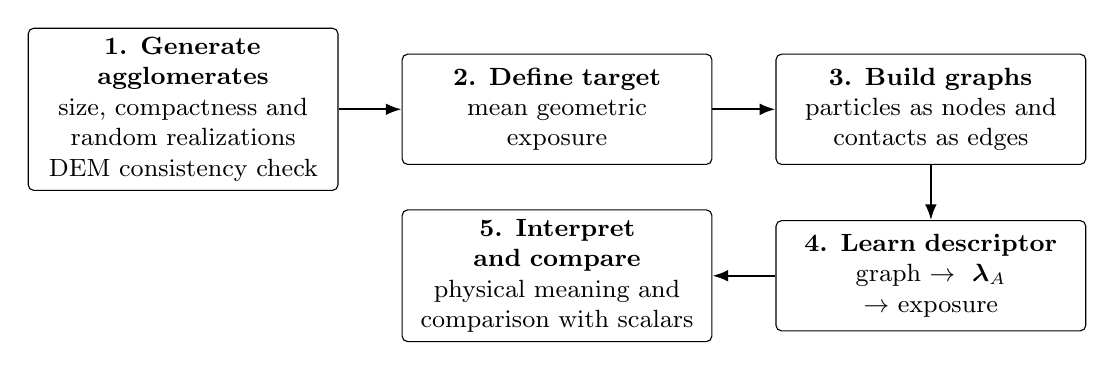
\begin{tikzpicture}[
		node distance=7mm and 8mm,
		workflowbox/.style={
			draw,
			rounded corners=2pt,
			align=center,
			minimum height=14mm,
			text width=3.7cm,
			font=\small
		},
		arrow/.style={-{Latex[length=2mm]}, thick}
	]
		\node[workflowbox] (generation) {
			\textbf{1. Generate agglomerates}\\
			size, compactness and\\random realizations\\DEM consistency check
		};
		\node[workflowbox, right=of generation] (targets) {
			\textbf{2. Define target}\\
			mean geometric\\exposure
		};
		\node[workflowbox, right=of targets] (graphs) {
			\textbf{3. Build graphs}\\
			particles as nodes and\\contacts as edges
		};
		\node[workflowbox, below=of graphs] (compression) {
			\textbf{4. Learn descriptor}\\
			graph $\rightarrow \boldsymbol{\lambda}_A$\\$\rightarrow$ exposure
		};
		\node[workflowbox, left=of compression] (interpretation) {
			\textbf{5. Interpret and compare}\\
			physical meaning and\\comparison with scalars
		};

		\draw[arrow] (generation) -- (targets);
		\draw[arrow] (targets) -- (graphs);
		\draw[arrow] (graphs) -- (compression);
		\draw[arrow] (compression) -- (interpretation);
	\end{tikzpicture}
	\caption{Five-step workflow for generating synthetic agglomerates, representing them as graphs, learning a compact structural descriptor and evaluating its physical meaning and predictive value. DEM is an auxiliary consistency check within generation, not a separate characterization step. The learning and comparison stages remain pending for the new dataset.}
	\label{fig:workflow}
\end{figure}

\subsection{Study design and agglomerate generation}
The ensemble contains $3\times4\times15=180$ independent geometries (Table~\ref{tab:database}).
\begin{table}[htbp]
\centering\small
\caption{Construction of the 180-agglomerate database. Every case has its own seed, coordinate file, contact list and metadata entry.}\label{tab:database}
\begin{tabular}{@{}p{0.21\linewidth}p{0.20\linewidth}p{0.39\linewidth}r@{}}\toprule
Growth method & Particle counts & Realizations per particle count & Cases\\\midrule
BPCA & 50, 100, 200, 500 & 15 independent seeds & 60\\
Balanced BCCA & 50, 100, 200, 500 & 15 independent seeds & 60\\
Local filling & 50, 100, 200, 500 & 3 detector radii $\times$ 5 seeds & 60\\\midrule
Total & 4 sizes & 45 geometries per size & 180\\\bottomrule
\end{tabular}
\end{table}
 The three growth methods are ballistic particle--cluster aggregation (BPCA), balanced ballistic cluster--cluster aggregation (BCCA), and local-filling growth. The particle counts are $N=50$, 100, 200 and 500, with 15 realizations for each method and size. Every particle has diameter $d=1\,\mu\mathrm{m}$.

BPCA adds one particle at a time along a randomly oriented straight trajectory, stopping at first contact. The collision search rejects trajectories that miss the cluster. BCCA recursively partitions the target particle number into two nearly equal groups, constructs those clusters, and joins them along a straight trajectory at first contact. Local-filling growth counts neighbours around each existing particle, selects a least-crowded attachment site and accepts an isotropic touching placement only if it creates no overlap; detector radii of 3, 6 and 12 particle radii are used, with five independent seeds per setting. Each algorithm defines a general growth mechanism and therefore helps control the range of structures produced. It does not uniquely prescribe the compactness or exposure of each realization; these properties must be measured from the generated coordinates. This differs from the earlier tunable fractal-like construction, which targeted a prescribed mass--radius relation~\cite{Filippov2000,Skorupski2014}. The current mechanisms do not impose $D_f$ or $k_f$. Dense-cluster generation is a separate extension~\cite{Ehrl2009}, not a property established by the name local filling. \pending{Add the original source for the specific local-filling implementation and concise pseudocode; distinguish the implementation from related published growth methods.}

Within each method and particle count, the 15 geometries are ranked by $N^{1/3}/(R_g/r)$, where $r=d/2$. The lowest, middle and highest five are labelled open, intermediate and compact. This is a rank-based division into three equal-sized groups, not an unsupervised clustering algorithm such as $k$-means. Here aggregation describes how particles are assembled; morphology grouping describes how the resulting structures are labelled. The labels are not ML prediction inputs. These labels are relative to that method and size; they are not common porosity thresholds across the ensemble. Continuous measured properties are used for comparisons across methods. The generation methods create tree-like initial contact networks, with $N-1$ contacts. This restricts the range of connectivity studied. The planned primary ML dataset contains these 180 geometries, representing 38,250 particles in total; no larger final sample count is claimed. A learning curve using increasing training subsets will show whether performance has stabilized and whether further geometries are needed.
\begin{figure}[p]
\centering
\newcommand{\snapshotbox}[2]{\fcolorbox{red}{white}{\parbox[c][30mm][c]{0.27\linewidth}{\centering\color{red}\small #1\\[2mm]#2\\[2mm][Snapshot to be inserted]}}}
\begin{tabular}{ccc}
\snapshotbox{BPCA}{Relatively open} & \snapshotbox{BPCA}{Intermediate} & \snapshotbox{BPCA}{Relatively compact}\\[4mm]
\snapshotbox{BCCA}{Relatively open} & \snapshotbox{BCCA}{Intermediate} & \snapshotbox{BCCA}{Relatively compact}\\[4mm]
\snapshotbox{Local filling}{Relatively open} & \snapshotbox{Local filling}{Intermediate} & \snapshotbox{Local filling}{Relatively compact}
\end{tabular}
\caption{Reserved panels for representative agglomerates from each growth method and measured compactness class, at a common particle count. Open and compact refer to within-method rankings, not universal density thresholds. \pending{Select cases from the manifest; label case ID, particle count and compactness score. Use the same camera convention and spatial scale, colour particles by exposure with a common 0--1 scale, and add a shared colour bar.}}
\label{fig:snapshots}
\end{figure}


\subsection{Auxiliary DEM consistency check}
The generator already checks connectivity and non-overlap. Bonded discrete-element method (DEM) calculations provide an additional numerical check of the response to a small mechanical disturbance; DEM is not required to build the graph or calculate exposure. Permanent rotational bonds join the initial contacts, and numerical drag damps prescribed small translational and rotational velocities. All 180 cases retain snapshots at $0$, $1$ and $2\,\mu\mathrm{s}$. Checks quantify particle displacement after removing rigid motion, size change, overlap, energy decay and preservation of particle and bond identities. The illustrative mechanical parameters are not fitted to a material. Full model settings and acceptance limits are given in Appendix~\ref{app:dem}. Learning before and after DEM will be compared on identical test splits.

\subsection{Geometric exposure as the prediction target}
For each particle, $M=512$ approximately uniform surface directions are constructed using a Fibonacci distribution. The Fibonacci construction distributes directions over the sphere using a constant golden-angle increment and evenly spaced heights~\cite{Gonzalez2010}. For $k=0,\ldots,M-1$, the implementation uses
\begin{equation}
 z_k=1-\frac{2(k+1/2)}{M},\quad \phi_k=k\pi(3-\sqrt{5}),\quad
 \boldsymbol{s}_k=\left(\sqrt{1-z_k^2}\cos\phi_k,\sqrt{1-z_k^2}\sin\phi_k,z_k\right).
\end{equation}
Fibonacci sampling specifies the ray directions; the subsequent ray--sphere intersection test determines whether each ray is blocked. These are separate steps. HEALPix provides a different, hierarchical equal-area discretization of the sphere~\cite{Gorski2005}. The present implementation uses Fibonacci sampling for a simple deterministic direction set with selectable point count; no superiority over HEALPix is assumed. \pending{Compare Fibonacci and HEALPix at comparable angular resolutions, including rotated configurations, before closing the sampling-sensitivity assessment.}

A ray starts just outside the surface and travels along the outward normal (Fig.~\ref{fig:ray_tracing_exposure}). Let $b_{im}=1$ if another particle blocks direction $m$ from particle $i$, and zero otherwise. Particle exposure and mean agglomerate exposure are
\begin{equation}
 a_i=1-\frac{1}{M}\sum_{m=1}^{M}b_{im},\qquad
 \overline a_{\mathrm{geo}}=\frac{1}{N}\sum_{i=1}^{N}a_i.
\end{equation}
Both lie between zero and one. A larger value means that more outward directions are unobstructed. This is a surface-normal visibility measure, rather than an integration over all directions from every surface point. It is not a diffusion calculation. Uniformly scaling all coordinates and radii leaves it unchanged. Here ``geometric proxy'' means a deliberately simplified geometric measure, not a validated replacement for a transport calculation. Interior particles contribute to the mean in the same way as boundary particles; it is not a measure of only the external envelope. A distant particle can obstruct a ray even when it is not in contact with the tested particle. This is the wider structural information the graph representation is intended to capture.
\begin{figure}[!tbp]
	\centering
	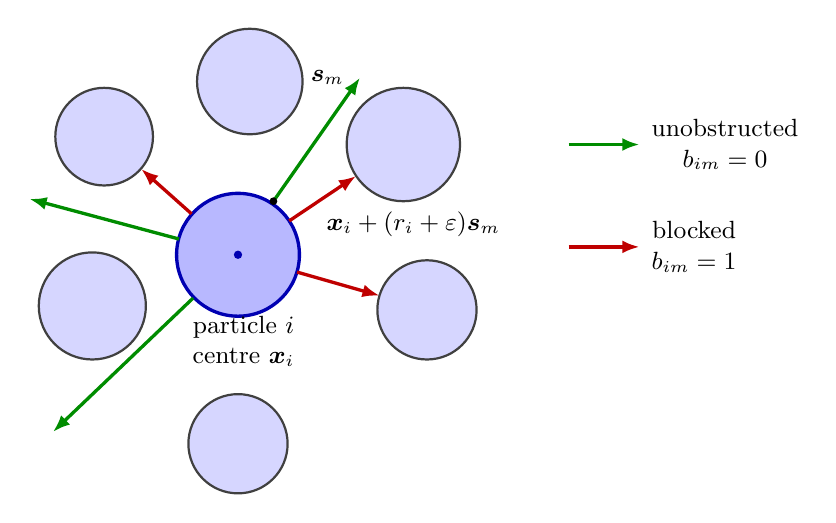
\begin{tikzpicture}[
		x=1cm,y=1cm,
		particle/.style={draw=black!75,thick,fill=blue!16},
		tested/.style={draw=blue!70!black,very thick,fill=blue!28},
		clear ray/.style={-{Latex[length=2.2mm]},very thick,green!55!black},
		blocked ray/.style={-{Latex[length=2.2mm]},very thick,red!75!black},
		label text/.style={font=\small,align=center}
	]
		% Neighbouring particles are drawn first so that the rays remain visible.
		\foreach \x/\y/\r in {
			4.55/0.55/0.63,
			4.25/2.65/0.72,
			2.30/3.45/0.67,
			0.45/2.75/0.62,
			0.30/0.60/0.68,
			2.15/-1.15/0.63}
			\draw[particle] (\x,\y) circle (\r);

		% Particle whose exposure is evaluated.
		\coordinate (C) at (2.15,1.25);
		\draw[tested] (C) circle (0.78);
		\fill[blue!70!black] (C) circle (1.5pt);
		\node[label text,below right=6.5mm and -7mm of C]
			{particle $i$\\centre $\boldsymbol{x}_i$};

		% Unobstructed rays extend into the surroundings.
		\draw[clear ray] (2.6,1.93) -- (3.70,3.50);
		\draw[clear ray] (1.40,1.45) -- (-0.50,1.96);
		\draw[clear ray] (1.58,0.70) -- (-0.20,-1.00);

		% Blocked rays stop at the first neighbouring particle.
		\draw[blocked ray] (2.90,1.03) -- (3.95,0.73);
		\draw[blocked ray] (2.80,1.68) -- (3.65,2.25);
		\draw[blocked ray] (1.56,1.77) -- (0.92,2.34);

		% Ray-start offset and direction annotation.
		\fill[black] (2.6,1.93) circle (1.4pt);
		\node[label text,above right=1mm and 10mm of C,shift={(0,0)}]
			{$\boldsymbol{x}_i+(r_i+\varepsilon)\boldsymbol{s}_m$};
		\node[label text,right] at (2.95,3.5) {$\boldsymbol{s}_m$};

		% Compact legend.
		\draw[clear ray] (6.35,2.65) -- (7.25,2.65);
		\node[label text,right] at (7.28,2.65)
			{unobstructed\\$b_{im}=0$};
		\draw[blocked ray] (6.35,1.35) -- (7.25,1.35);
		\node[label text,right] at (7.28,1.35)
			{blocked\\$b_{im}=1$};
	\end{tikzpicture}
	\caption{Schematic of the ray-tracing calculation for one particle $i$.
		Rays start just outside its surface and follow sampled outward directions
		$\boldsymbol{s}_m$. A ray is blocked when it intersects another particle;
		otherwise, it contributes to the exposed fraction. For clarity, only a
		two-dimensional section and a small subset of rays are shown; the actual
		calculation distributes $M=512$ directions over the complete sphere.}
	\label{fig:ray_tracing_exposure}
\end{figure}


Exposure is calculated for all three stored snapshots. The final configuration is the planned primary sample for learning, giving 180 independent samples. The intermediate times are used to inspect changes during DEM, not to increase the apparent sample count. Particle geometry and exposure are stored together for visualization. A 2048-ray comparison on three representative 500-particle cases checks sensitivity to angular resolution.

\subsection{Conventional structural descriptors}
The comparison follows the six descriptors used in the earlier report (Table~\ref{tab:descriptors}). Here $\boldsymbol{x}_c$ is the mean particle centre, and $z_i$ is the number of neighbours connected to particle $i$. For identical spheres, the size measure includes the particles' own contribution to their mass distribution:
\begin{equation}
 R_g^2=\frac{1}{N}\sum_i\lVert\boldsymbol{x}_i-\boldsymbol{x}_c\rVert^2+\frac{3r^2}{5}.
\end{equation}
\begin{table}[htbp]
\centering\small
\caption{The same six conventional inputs will be supplied to linear regression, random forest and ANN models.}\label{tab:descriptors}
\begin{tabular}{@{}lp{0.71\linewidth}@{}}\toprule
Descriptor & Plain-language meaning\\\midrule
$N$ & Number of primary particles.\\
$R_g/d$ & Spread of particle mass around the centre, normalized by particle diameter.\\
$N_c$ & Number of unique particle connections, counting each pair once.\\
$\rho_c=2N_c/[N(N-1)]$ & Fraction of all possible particle pairs that are connected.\\
$\overline z=2N_c/N$ & Mean number of connected neighbours per particle.\\
$z_{\max}$ & Largest number of connected neighbours of any particle.\\\bottomrule
\end{tabular}
\end{table}

The exact rule for identifying connections in the final geometry must be fixed before training and used consistently for graphs and descriptors. Permanent mechanical bonds and geometrical contacts are not automatically identical. \pending{Specify and verify the final contact tolerance, treatment of slightly separated bonded pairs, and consistency with the earlier report's radius-of-gyration convention.}

\subsection{Prediction models and learned structural parameters}
Linear regression combines descriptors through a weighted sum. A random forest combines several decision trees and can represent nonlinear relationships. An artificial neural network (ANN) passes the six descriptors through successive layers of adjustable calculations to predict exposure. Its weights are learned from examples. Unlike linear regression, it can learn nonlinear combinations of the same conventional information.

The graph neural network (GNN) receives the detailed particle graph instead of the six aggregate descriptors. Particle properties are attached to nodes, and pair properties are attached to links. Successive network layers exchange information along the links, allowing each particle's representation to include information about its neighbourhood. A final aggregation step combines particle information into one representation of the agglomerate.

The \emph{latent vector},
\begin{equation}
 \boldsymbol{\lambda}=(\lambda_1,\ldots,\lambda_q),
\end{equation}
is simply a short list of $q$ learned, artificial structural parameters. These parameters are alternatives to prescribed descriptors such as size and coordination. The network chooses them so that, together, they help predict geometric exposure. They are not guaranteed to describe every aspect of structure, and each number need not correspond to one familiar physical property. With $q=1$, the structure is summarized by one learned number. A small prediction network uses only this vector to estimate exposure; no separate structural inputs bypass it.

The planned graph model follows the earlier report's geometry-aware architecture: six graph layers, 64 internal features and a comparison of different vector lengths. The earlier implementation must be recovered or reconstructed and checked before the settings are treated as final. The GNN includes both a learned characterization step and a prediction step, trained together. To separate representation quality from prediction-model complexity, the planned study will supplement the independently tuned six-descriptor ANN with a controlled comparison: six descriptors pass through a learned map to $q$ parameters, followed by the same prediction-head architecture used after the GNN vector. Both routes will use the same loss, output activation and training-side selection budget. Encoder parameter counts, total trainable weights and training cost will be reported separately; an identical head does not make the encoders equally complex. \pending{Implement the matched-head comparison and document its capacity and tuning budget before reporting an advantage for the graph representation.}

The ANN size and regularization, which limits excessive fitting to the training samples, will be selected using training-side validation. \pending{Add the verified node and link inputs, graph-layer equations, ANN architecture, parameter counts, optimization settings and candidate vector lengths after implementation.}

\subsection{Software and model implementation}
Table~\ref{tab:software} separates verified computational software from the planned learning stack. The generation and exposure scripts use Python and NumPy; local DEM results used LAMMPS 22 July 2025, Update 4. The reproducible runner environment pins NumPy 2.3.5, the LAMMPS Python distribution 2025.7.22.4.0, and MPICH 5.0.1.post1. These pins describe the environment specification, not a claim that remote validation has finished.
\begin{table}[htbp]
\centering\small
\caption{Computational tools and planned learning models. ML entries specify the intended implementation; final versions and settings remain pending.}\label{tab:software}
\begin{tabular}{@{}p{0.23\linewidth}p{0.25\linewidth}p{0.43\linewidth}@{}}\toprule
Task / model & Python library / engine & Function and details to report\\\midrule
Geometry and exposure & NumPy; Python standard library & Arrays, ray intersection tests, CSV/JSON case records.\\
Bonded DEM & LAMMPS; MPICH runtime & Particle translation, rotation, bonds and contacts.\\
Linear regression & scikit-learn (planned) & Weighted sum of six descriptors; report scaling and intercept.\\
Random forest & scikit-learn (planned) & Nonlinear ensemble of trees; report tree count, depth and leaf settings.\\
Six-descriptor ANN & PyTorch (planned) & Fully connected nonlinear model; report layer widths, activations, regularization and optimizer.\\
GNN & PyTorch and PyTorch Geometric (planned) & Particle-neighbour information exchange, pooling, learned vector and prediction head; verify six layers and 64 internal features.\\
Analysis and plots & pandas, SciPy, Matplotlib (planned) & Tabulation, statistics, prediction plots and learning curves.\\\bottomrule
\end{tabular}
\end{table}

\pending{After recovering the training code, record Python and every ML library version, hardware, CPU/GPU use, runtime, random seeds and environment lock file. The existing interpretation script imports PyTorch, PyTorch Geometric and scikit-learn, but this is not evidence that the new 180-case models have been trained.}

\subsection{Training, validation and model comparison}
The model learns from a training set. A validation set guides choices such as network size and when to stop training. A test set evaluates prediction on agglomerates that were not used for either purpose. Scaling of inputs is calculated only from training samples and then applied to the withheld samples. The target exposure is never an input.

In five-fold cross-validation, the data are divided into five parts, called folds. Each part is withheld once while the model is developed using the other four. An \emph{out-of-fold prediction} is therefore a prediction for an agglomerate made by a model that did not use that agglomerate for training or model selection. Collecting these predictions produces one independently evaluated prediction per sample. This is more informative about generalization than showing agreement on samples used for fitting.

All models will use identical outer test folds. Choices of architecture, vector length, scaling and stopping time will be made using further splits inside the training portion, not the outer test predictions. Related versions of an agglomerate, including snapshots or rotated copies, must stay together. Primary folds will hold out generation-setting groups, defined by method, particle count and the detector setting where applicable. Additional tests will withhold an entire generation method and, separately, train on smaller agglomerates and test on $N=500$. These tests address different questions and will be reported separately. \pending{Freeze and publish the exact split manifest, inner validation rules and random seeds before fitting.}

Training curves will show how error changes as model weights are updated. Several random initializations will quantify how much the neural-network results depend on their starting weights. A final model may subsequently be fitted to all data for use and structural interpretation, but its training agreement will not replace the withheld-data evaluation.

\subsection{Error measures and interpretation}
For $n$ withheld samples with calculated exposures $y_j$ and predictions $\widehat y_j$, the reported measures are
\begin{align}
 \mathrm{RMSE}&=\sqrt{\frac{1}{n}\sum_j(\widehat y_j-y_j)^2},\\
 \mathrm{MAE}&=\frac{1}{n}\sum_j|\widehat y_j-y_j|,\\
 R^2&=1-\frac{\sum_j(y_j-\widehat y_j)^2}{\sum_j(y_j-\overline y)^2}.
\end{align}
RMSE emphasizes larger errors, whereas MAE is the average absolute error. Lower values are better. $R^2=1$ indicates perfect prediction; negative values are possible and indicate performance worse than predicting the mean of the evaluated targets. A separate baseline that always predicts the training-set mean will also be reported. Error is expressed in exposure units: an MAE of 0.02 means an average error of two percentage points in exposure. Prediction quality will also be judged against the spread of exposures in the dataset, the training-mean baseline, the angular-discretization sensitivity and paired differences between models on the same withheld agglomerates. A high $R^2$ alone does not establish engineering relevance.

The learned parameters will be compared with conventional descriptors using scatter plots and correlations. Their ability to be reconstructed from those descriptors will also be examined. Correlation means that quantities vary together; it does not establish a physical cause. Learned coordinates can change sign or scale between independently trained networks. Interpretation will account for this ambiguity and will be distinguished from independent predictive evaluation.

\section{Results}
\subsection{Generated structures and DEM checks}
All 180 locally computed cases met the stated numerical checks, retaining exactly three particle snapshots and three bond snapshots. Across the ensemble, final-to-initial kinetic-energy ratios ranged from $3.89\times10^{-6}$ to $2.15\times10^{-5}$. The largest displacement after removing rigid motion was $2.95\times10^{-5}d$, and the largest particle overlap was $9.30\times10^{-8}d$. The maximum absolute relative change in radius of gyration was $3.95\times10^{-6}$ (rounded upwards). Thus the chosen perturbation produced only small changes in these configurations. These numbers refer to the archived local campaign; independent runner validation is reported separately when complete.

\subsection{Distribution and numerical resolution of exposure}
The final-snapshot results are summarized in Table~\ref{tab:exposure}. Each row includes all four particle counts. Differences between rows therefore describe the sampled ensembles, rather than a universal ordering of the generation algorithms. In particular, the name local filling should not be interpreted as guaranteeing lower exposure than every other method.
\begin{table}[htbp]
\centering
\caption{Mean geometric exposure at the final DEM snapshot, calculated with 512 rays per particle. Each method contributes 60 agglomerates.}\label{tab:exposure}
\begin{tabular}{@{}lrrr@{}}\toprule
Method & Minimum & Maximum & Ensemble mean\\\midrule
BPCA & 0.3933 & 0.6498 & 0.5259\\
BCCA & 0.5452 & 0.7287 & 0.6419\\
Local filling & 0.5359 & 0.7458 & 0.6599\\\bottomrule
\end{tabular}
\end{table}

For one 500-particle case per method, increasing the ray count from 512 to 2048 changed the agglomerate mean by less than $4.50\times10^{-4}$. Individual particle values changed by up to about 0.0274. This limited check supports the reported mean values for those cases, but is not a convergence bound for all geometries. \pending{Add representative images coloured by particle exposure and distributions resolved by method and particle count.}

\subsection{Prediction accuracy and comparison with conventional descriptors}
\pending{Training on the 180-case dataset has not yet been completed. Populate Table~\ref{tab:ml} from the saved out-of-fold predictions; add predicted-versus-calculated plots, per-fold errors and variability across training seeds.}
\begin{table}[htbp]
\centering\small
\caption{Planned comparison on identical withheld samples. Dashes indicate results not yet available, not zero error.}\label{tab:ml}
\begin{tabular}{@{}p{0.52\linewidth}rrr@{}}\toprule
Model and input & RMSE & MAE & $R^2$\\\midrule
Training-mean baseline & --- & --- & ---\\
Linear regression, six descriptors & --- & --- & ---\\
Random forest, six descriptors & --- & --- & ---\\
ANN, six descriptors & --- & --- & ---\\
GNN, particle graph & --- & --- & ---\\\bottomrule
\end{tabular}
\end{table}

\subsection{Number and meaning of learned parameters}
\pending{Add the vector-length comparison, selection stability across folds, training curves, learned-parameter correlations and reconstruction from conventional descriptors. Do not select a vector length using the final test errors.}

\subsection{Influence of the DEM consistency step}
\pending{Train the same models on the initial generated geometries and on the final DEM geometries using identical agglomerate IDs, splits and tuning rules. Report the change in mean exposure, descriptor values and prediction errors. This directly tests whether DEM affects the conclusions; small displacements alone do not replace this comparison.}

\subsection{Prediction for new sizes and growth methods}
\pending{Report the method-holdout and 500-particle tests separately from the primary five-fold results, including error distributions and any failure cases.}

\section{Discussion}
The decisive comparison is between the GNN and the ANN using six descriptors. Both can learn nonlinear relationships, but only the GNN receives the detailed graph. Better GNN predictions on the same withheld samples would support the value of that additional structural information for this target. Similar performance would support using the simpler descriptor-based model within the studied range. Neither outcome should be assumed before the comparison is completed.

There are important limits to this interpretation. Several conventional descriptors are mathematically related: $\overline z=2N_c/N$ and $\rho_c=\overline z/(N-1)$. With a tree network, $N_c=N-1$, so much of their variation is determined by particle count. The six inputs are retained for continuity with the earlier report, but they are not six independent structural measurements. A weak baseline on this ensemble alone would not establish that all conventional descriptors are inadequate.

The generated structures span three growth mechanisms but do not cover dense networks with many loops. Permanent bonds preserve the initial connectivity, and the selected perturbation is deliberately small. Material parameters have not been calibrated against experiments. The graph can represent non-self-similar arrangements, but this ability is not evidence of predictive generalization to every such structure. Local porosity and non-contact geometric proximity may influence shielding without being fully captured by a finite number of contact-graph layers. These limitations motivate the method-holdout tests and future more varied structures.

Fractal-dimension measurements require care for small finite clusters and depend on the method and available scaling range~\cite{Bushell2002,Theiler1990}. Box-counting implementations introduce additional resolution choices~\cite{ForoutanPour1999,Liebovitch1989}. The earlier report's radial 10--80\% fitting window was an analysis choice, not asserted here as a universal standard. No reliable fractal dimension is required or claimed for the current geometries. If such estimates are added descriptively, fitting-window sensitivity and the actual scaling interval must be reported. Overall DEM changes are instead quantified directly through aligned displacement, radius of gyration, overlap and energy. The exposure target itself is a geometric measure and excludes fluid motion, diffusion and reaction. Any extension to uptake requires separate transport calculations or experiments.

The earlier 135-agglomerate study is a distinct dataset. Its reported prediction scores are not results for the present 180-case ensemble and are not entered in Table~\ref{tab:ml}. Likewise, its prescribed fractal-dimension and prefactor baseline cannot be transferred directly to algorithms that do not use those same controls. Future work could test mass and heat transfer, diffusion, reaction or optical response in particle agglomerates. These are outlook applications, not validation provided by the current exposure target. \pending{Extend the discussion after training: effect size, uncertainty, model complexity and practical implications. Decide the target journal from the demonstrated contribution rather than implying transport validation from a geometric test.}

\section{Conclusions}
A reproducible ensemble of 180 agglomerates has been generated and assessed with bonded DEM. Particle-level geometric exposure and three snapshots per agglomerate are available for analysis and visualization. The manuscript defines a comparison between graph-based learned parameters and conventional descriptors, including a nonlinear ANN using the same six descriptors as the existing baselines. \pending{Complete the conclusions after training: answer the research question quantitatively, state the supported number of learned parameters, and delimit the range of applicability.}

\section*{Data and code availability}
Generation, DEM and exposure-analysis code, generated coordinates and local numerical summaries are maintained in \url{https://github.com/khalifali/PrelimDFG_GNN}. The current source summaries are in \texttt{results/study180/}; model splits, training code, prediction files and checkpoints will be added when available. \pending{Add the immutable release identifier and permanent archive for submission.}
\section*{Author contributions, funding and competing interests}
\pending{To be completed and confirmed by the authors.}
\FloatBarrier
\appendix
\section{Bonded DEM setup and numerical checks}\label{app:dem}
The discrete-element method follows the translation and rotation of individual particles under applied forces and torques. The present calculations use LAMMPS, with spherical particles and rotational bonds connecting the initial contacts. The bonds resist extension, shear, bending and twisting. They do not break, and no new permanent bonds are formed. Unbonded neighbours interact through Hertz--Mindlin repulsive contacts; the repulsive contact model is not added again to bonded pairs.

The generated geometry defines the stress-free bond reference. Small reproducible random translational and angular velocities perturb this configuration, with total linear and angular momentum removed. Numerical drag then dissipates motion. The generator already checks connectivity and non-overlap; DEM is therefore an auxiliary mechanical consistency check, not a prerequisite for constructing a graph or calculating exposure. This tests the implemented mechanical response near the chosen configuration; it does not show that the structure would arise naturally or survive arbitrary loading. The parameters in Tables~\ref{tab:particles} and~\ref{tab:contacts} are illustrative rather than fitted to a material.

\begin{table}[htbp]
\centering\small
\caption{Particle properties and numerical settings. All particles are identical spheres; mechanical parameters are illustrative. Velocity scales precede momentum removal.}\label{tab:particles}
\begin{tabular}{@{}p{0.57\linewidth}p{0.35\linewidth}@{}}\toprule
Quantity & Value\\\midrule
Diameter; density & $1\,\mu\mathrm{m}$; $1050\,\mathrm{kg\,m^{-3}}$\\
Mass $m=\rho\pi d^3/6$ & $5.50\times10^{-16}\,\mathrm{kg}$\\
Moment of inertia $I=md^2/10$ & $5.50\times10^{-29}\,\mathrm{kg\,m^2}$\\
Initial translational velocity scale & $10^{-3}\,\mathrm{m\,s^{-1}}$ per component\\
Initial angular velocity scale & $1000\,\mathrm{rad\,s^{-1}}$ per component\\
Translational numerical drag & $10^{-8}\,\mathrm{kg\,s^{-1}}$\\
Rotational numerical drag & $10^{-22}\,\mathrm{kg\,m^2\,s^{-1}}$\\
Time step; duration & $10^{-10}\,\mathrm{s}$; $2\,\mu\mathrm{s}$\\
Stored snapshots per case & $0$, $1$, $2\,\mu\mathrm{s}$\\\bottomrule
\end{tabular}
\end{table}
\begin{table}[htbp]
\centering\small
\caption{Mechanical connections and contact properties. Permanent bonds and unbonded repulsive contacts have distinct roles.}\label{tab:contacts}
\begin{tabular}{@{}p{0.57\linewidth}p{0.35\linewidth}@{}}\toprule
Model or property & Setting\\\midrule
LAMMPS particle / integration styles & \texttt{bpm/sphere}; \texttt{nve/bpm/sphere}\\
Permanent bond style & \texttt{bpm/rotational}\\
Bond normal / shear stiffness & $10 / 4\,\mathrm{N\,m^{-1}}$\\
Bond twist / bend stiffness & $10^{-13} / 10^{-13}\,\mathrm{N\,m}$\\
Bond normal / shear damping & $10^{-8} / 10^{-8}\,\mathrm{kg\,s^{-1}}$\\
Bond twist / bend damping & $10^{-22} / 10^{-22}\,\mathrm{kg\,m^2\,s^{-1}}$\\
Unbonded repulsion & Hertz--Mindlin\\
Young's modulus; Poisson ratio & $10^9\,\mathrm{Pa}$; $0.3$\\
Restitution; sliding friction & $0.5$; $0.3$\\
Bond breaking / later bond formation & Both disabled\\
van der Waals attraction & Disabled\\
Stress-free reference & Initial generated configuration\\\bottomrule
\end{tabular}
\end{table}


Acceptance checks require finite outputs, unchanged particle and bond identities, maximum overlap below $0.1\%$ of the diameter, displacement below $1\%$ of the diameter after removing rigid translation and rotation, and final kinetic energy below $0.1\%$ of its initial value. Kinetic energy includes translation and rotation. These are numerical checks, not experimental material validation. A stationary control and a time-step refinement comparison are available for one 500-particle case from each generation method.


\FloatBarrier
\bibliographystyle{plainnat}
\bibliography{references_agglomerate_exposure}
\end{document}
